\PassOptionsToPackage{naturalnames}{hyperref}
\RequirePackage{luatex85}
\documentclass{article}
\usepackage{geometry}
%\usepackage{fullpage}
\usepackage{parskip}
\usepackage{physics}
\usepackage{amsmath}
\usepackage{amssymb}
\usepackage{xcolor}
\usepackage[colorlinks,linkcolor=blue,citecolor=green]{hyperref}
\usepackage{array}
\usepackage{longtable}
\usepackage{multirow}
\usepackage{comment}
\usepackage{graphicx}
\usepackage{cite}
\usepackage{amsfonts}
\usepackage{bm}
\usepackage{slashed}
\usepackage{dsfont}
\usepackage{mathtools}
\usepackage[compat=1.1.0]{tikz-feynman}
\usepackage{simplewick}
%\usepackage{fourier}
%\usepackage{slashbox}
%\usepackage{intent}
\usepackage{mathrsfs}
\usepackage{xparse}
\usepackage{enumerate}
%\usepackage{axodraw4j}


\geometry{left=0.9cm,right=0.9cm,top=1.5cm,bottom=2cm}

\newcommand{\gm}{\gamma^{\mu}}
\newcommand{\gn}{\gamma^{\nu}}
\newcommand{\gs}{\gamma^{\sigma}}
\newcommand{\gr}{\gamma^{\rho}}
\newcommand{\gnr}{g^{\nu\rho}}
\newcommand{\gmr}{g^{\mu\rho}}
\newcommand{\gms}{g^{\mu\sigma}}
\newcommand{\gns}{g^{\nu\sigma}}
\newcommand{\vbp}{\vb{p}}
\newcommand{\vbk}{\vb{k}}
\newcommand{\g}{\gamma}
\renewcommand{\a}{\alpha}
\renewcommand{\b}{\beta}
\renewcommand{\t}{\theta}
\newcommand{\la}{\lambda}
\newcommand{\p}{\phi}
\newcommand{\vp}{\varphi}
\newcommand{\s}{\sigma}
\newcommand{\G}{\Gamma}
\newcommand{\pars}{\slashed\partial}
\newcommand{\ps}{\slashed p}
\newcommand{\ks}{\slashed k}
\newcommand{\lag}{\mathcal{L}}
\newcommand{\da}{^{\dagger}}
\newcommand{\sm}{^{\mu}}
\newcommand{\sn}{^{\nu}}
\newcommand{\smn}{^{\mu\nu}}
\newcommand{\Dm}{D^{\mu}}
\newcommand{\dm}{\partial^{\mu}}
\newcommand{\Asquare}{A^{\mu}A_{\mu}}
\newcommand{\partialsquare}[2]{\partial^{\mu}{#1}\partial_{\mu}{#2}}

\title{Local Operator divergence}
\author{Yingsheng Huang}
\begin{document}
\maketitle
NRQED matrix element
\begin{align*}
  &-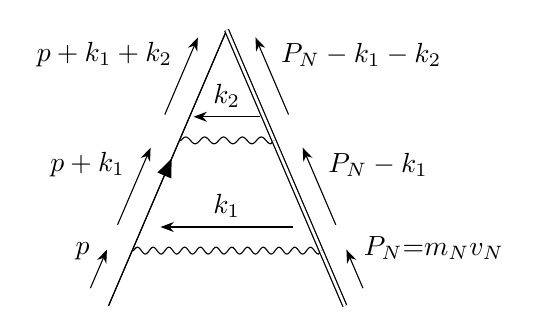
\begin{tikzpicture}[baseline=($(p1)!0.5!(x)$)]
 \begin{feynman}
   \vertex (p1);
 \vertex[right=3cm of p1] (p2);
 \vertex at ($(p1)!0.5!(p2)+(0,3.5cm)$) (x) ;
 \vertex at ($(p1)!0.2!(x)$) (y1);
 \vertex at ($(p2)!0.2!(x)$) (z1);
 \vertex at ($(p1)!0.6!(x)$) (y2);
 \vertex at ($(p2)!0.6!(x)$) (z2);
 %
 \diagram* {
   (p1) -- [fermion] (x);
   (p2) -- [double distance=1pt] (x);
   (y1) -- [photon,rmomentum=$k_1$] (z1);
   (y2) -- [photon,rmomentum=$k_2$] (z2);
   (p1) -- [momentum=\(p\)] (y1);
   (p2) -- [momentum'=$P_{N}\text{=}m_{N}v_{N}$,double distance=1pt] (z1);
   (y1) -- [momentum=\(p+k_1\)] (y2);
   (z1) -- [momentum'=\(P_{N}-k_1\),double distance=1pt] (z2);
   (y2) -- [momentum=\(p+k_1+k_2\)] (x);
   (z2) -- [momentum'=\(P_{N}-k_1-k_2\),double distance=1pt] (x);
   };
 \end{feynman}
 \end{tikzpicture}\\ =&e^4\int[dk_1][dk_2]\frac{1}{\vb{\abs{k_1}}^2}\frac{1}{\vb{\abs{k_2}}^2}\frac{1}{-k_1^0-k_2^0+i\epsilon}\frac{1}{-k_1^0+i\epsilon}\frac{1}{p^0+k_1^0-m-\frac{\vb{(p+k_1)}^2}{2m}+i\epsilon}\frac{1}{p^0+k_1^0+k_2^0-m-\frac{\vb{(p+k_1+k_2)}^2}{2m}+i\epsilon}\psi_e(p)u_N(v_N)
 \\
 \intertext{do the shift as above}
 =&-e^4\int\frac{\dd^3\vb{k_1}}{(2\pi)^3}\frac{\dd^3\vb{k_2}}{(2\pi)^3}\frac{1}{\vb{\abs{k_1-p}}^2}\frac{1}{\vb{\abs{k_2-k_1}}^2}\frac{1}{E-\frac{\vb{\abs{k_1}}^2}{2m}+2i\epsilon}\frac{1}{E-\frac{\vb{\abs{k_2}}^2}{2m}+2i\epsilon}\psi_e(p)u_N(v_N)\\
 \intertext{drop $\vb{p}$}
 =&-e^4\int\frac{\dd^3\vb{k_1}}{(2\pi)^3}\frac{\dd^3\vb{k_2}}{(2\pi)^3}\frac{1}{\vb{\abs{k_1}}^2}\frac{1}{\vb{\abs{k_2-k_1}}^2}\frac{1}{-\frac{\vb{\abs{k_1}}^2}{2m}+2i\epsilon}\frac{1}{-\frac{\vb{\abs{k_2}}^2}{2m}+2i\epsilon}\psi_e(p)u_N(v_N)
\end{align*}



\end{document}
